% 正文开始
% Chapter 1: Introduction
\section{Introduction}
\subsection{Problem Background}

%---------------------------------子图的排版与语法
\begin{figure}[htbp]
    \centering    
    \subfigure[Subfigure Name1(left)]{				% 图片1([]内为子图标题)						
    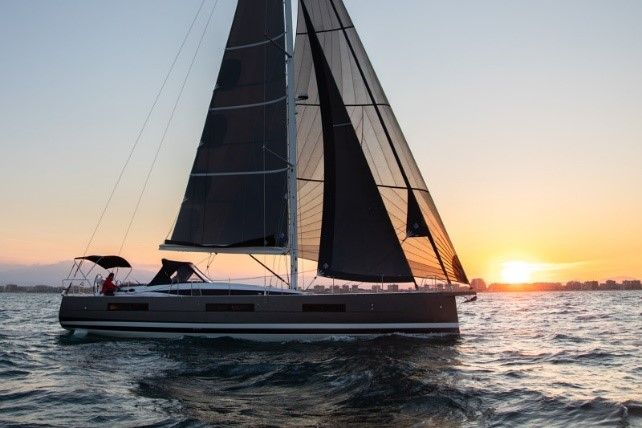
\includegraphics[width=0.45\textwidth]{test_1.jpg}}			  % 子图1的图片宽度 不能空行
    \subfigure[Subfigure Name2(right)]{				% 图片2,其中width代表图片宽度,可以调整
    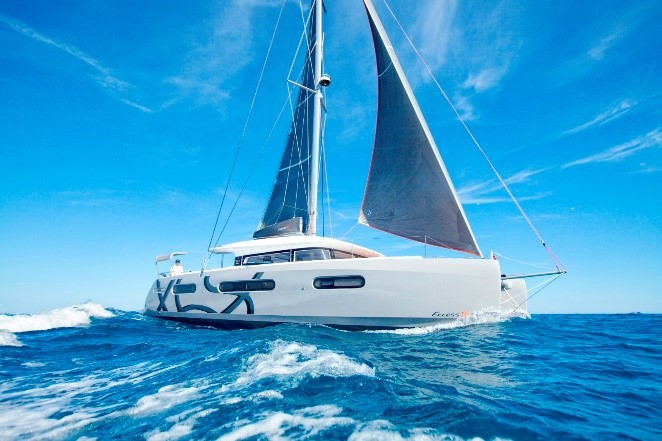
\includegraphics[width=0.45\textwidth]{test_2.jpg}} %注意此处的文件格式为.jpg
	\caption{Figure Name} % 图片标题 
\end{figure}
\vspace{-1cm} %下文向下空-1cm
\subsection{Restatement of the Problem}

%----------------------------------无序列表的排版与语法
\begin{itemize}
    \setlength{\parsep}{0ex} %段落间距
    \setlength{\topsep}{2ex} %列表到上下文的垂直距离
    \setlength{\itemsep}{1ex} %条目间距
    \item Problem 1: 
    \item Problem 2:
    \item Problem 3: 
    \item Problem 4\&5: 
\end{itemize}

%---------------------------------大图的排版与语法
\begin{figure}[H]  %h此处,t页顶,b页底,p独立一页,浮动体出现的位置
    \centering  %图表居中
    
\includegraphics[width=.80\textwidth]{cat.jpeg} %图片的名称或者路径之中有空格会出问题 
    \caption{Flow Chart of this Paper's Research} % 图片标题 
\end{figure}
\vspace{-1cm}

%--------------------------------假设部分较复杂的无序列表
\section{Assumptions and Explanations}
Considering ...
\begin{enumerate}[\bfseries \textit{Assumption} 1:]
	\item \textbf{We assume that ...}\\
	\textbf{\textit{Explanation:}}...
	\item \textbf{We assume that ...}\\
	\textbf{\textit{Explanation:}}...
	\item \textbf{We assume ...}\\
	\textbf{\textit{Explanation:}}...
\end{enumerate}

\section{Notations}
Some important mathematical notations used in this paper are listed in \Cref{tb:notations}. 
%上部对于table的处理使用了交叉引用可以实时更改序号
\begin{table}[H]
\begin{center}
\caption{Notations used in this paper}\label{tb:notations}
\begin{tabular}{c c c}
\toprule[2pt] %三线表顶端线宽度
\multicolumn{1}{m{1.5cm}}{\centering \textbf{Symbol}} %开始写表内容捏,其中{m{xxcm}}表示该列宽度
&\multicolumn{1}{m{12.5cm}}{\centering\textbf{Description} }
&\multicolumn{1}{m{1cm}}{\centering \textbf{Units}}\\
\midrule
$\lambda_i$& Meaning of the symbol&/ \\
$y_i$& Meaning of the symbol&/\\
$a_i$& Meaning of the symbol&/\\
$\Delta R$&Meaning of the symbol&/ \\
$R^*$ &Meaning of the symbol &/\\
\bottomrule[2pt]
\end{tabular}

\begin{tablenotes}%等等,表格还有些说明!
        \footnotesize
        \item[*] *There are some variables that are not listed here and will be discussed in detail in each section. %此处加入注释*信息
\end{tablenotes}
\end{center}
\end{table}
\vspace{-1.2cm}%在\end{table}下加一行\vspace{-1cm} 其中-1的作用是缩短与下方文字距离的 切记!必须是负数

\section{Model Preparation}
\subsection{Data Overview}
For a large amount of data, it is necessary to process and clean the data before building the model. So we first use the ismissing function to find the missing value and get the missing value in \Cref{tb:missing_data}:
\begin{table}[H]%浮动体的htbp可以强制在原位显示,改参数为H
  \begin{center}
  \fontsize{12pt}{13.8}
  \caption{Missing Data in Given Data} \label{tb:missing_data}
  \resizebox{\textwidth}{!}
  {\begin{tabular}{||l|l|c c c c|r|r||} %此处设置了不同类型的参数及线供参考
  \toprule[2pt]
  \multicolumn{1}{m{3cm}}{\centering \textbf{Missing1}} %大型表格需要好好斟酌每一列的宽度捏
  &\multicolumn{1}{m{2cm}}{\centering \textbf{Missing2}}
  &\multicolumn{1}{m{2cm}}{\centering \textbf{Missing3}}
  &\multicolumn{1}{m{2cm}}{\centering \textbf{Missing4}}
  &\multicolumn{1}{m{2cm}}{\centering \textbf{Missing5}}
  &\multicolumn{1}{m{2cm}}{\centering \textbf{Missing6}}
  &\multicolumn{1}{m{2cm}}{\centering \textbf{Missing7}}
  &\multicolumn{1}{m{2cm}}{\centering \textbf{Missing8}}
  \\ %m后面是列宽
  \midrule
  \multirow{3}*{\makecell[c]{Looooog\\Word}}%合并行操作,同时进行了合并行内的换行,{}内是合并的行数
  &A&B&C&D&-&E&F \\
  ~ &A&B&C&D&-&E&F   \\
  ~ &A&B&C&D&-&E&F \\ 
  Multicolumn&\multicolumn{7}{c}{These columns share common features} \\%合并列操作,{}内是合并的列数
  \bottomrule[2pt]
  \end{tabular}}
  \end{center}
\end{table}
\vspace{-1cm}

\subsubsection{Data Collection}
And other data sources are shown in \Cref{tb:data_source}.

\begin{table}[H]
    \begin{center}
    \caption{Data and Database Websites}\label{tb:data_source}
    \resizebox{\textwidth}{!}
    {\begin{tabular}{c c}
    \toprule[2pt]
    \multicolumn{1}{m{6.5cm}}{\centering \textbf{Database Names}}
    &\multicolumn{1}{m{10cm}}{\centering \textbf{Database Websites} }\\ %m后面是列宽
    \midrule
    GDP of Each Country& https://ourworldindata.org/ \\
    GDP of Some European Countries & https://data.worldbank.org/ \\
    \multirow{2}*{Partial Sailing Parameters}& https://www.sailboat-cruising.com/\\ 
    ~& https://sailboatdata.com/ \\
    \bottomrule[2pt]
    \end{tabular}}
    \end{center}
\end{table}
\vspace{-1cm}

\subsubsection{Data Screening}
According to the data given, we...
\begin{figure}[htbp]
    \centering    
    \subfigure[Cute Cat(left)]{									
    
\includegraphics[width=0.45\textwidth]{catsquare.jpeg}}			 
    \subfigure[Cute Cat(right)]{				
    
\includegraphics[width=0.45\textwidth]{catsquare.jpeg}} %此时两张图片的大小不一样就需要改width参数
	\caption{Data Screening}  
\end{figure}
\vspace{-1cm}

This is a double-table.

\begin{table}[H] %浮动体的htbp可以强制在原位显示,改参数为H
    \begin{center}
    \caption{Partial Monohull and Catamaran data}
    \resizebox{\textwidth}{!}
    {\begin{tabular}{c c c c c c}
    \toprule[2pt]
    \multicolumn{1}{m{4cm}}{\centering \textbf{AA}}
    &\multicolumn{1}{m{2cm}}{\centering \textbf{BB$/m$}}
    &\multicolumn{1}{m{2cm}}{\centering \textbf{CC/m$^3$}}
    &\multicolumn{1}{m{2cm}}{\centering \textbf{DD\\/m$^3$}}%此处如果DD过长可以使用\\换行
    &\multicolumn{1}{m{2cm}}{\centering \textbf{EE/m$^2$}}
    &\multicolumn{1}{m{4cm}}{\centering \textbf{FF}}
    \\ %m后面是列宽
    \midrule
    A&B&C&D&E&F \\
    A&B&C&D&E&F\\
    \bottomrule[2pt]
    \toprule[2pt]
    \multicolumn{1}{m{4cm}}{\centering \textbf{AA}}
    &\multicolumn{1}{m{2cm}}{\centering \textbf{BB$/m$}}
    &\multicolumn{1}{m{2cm}}{\centering \textbf{CC/m$^3$}}
    &\multicolumn{1}{m{2cm}}{\centering \textbf{DD\\/m$^3$}}%此处如果DD过长可以使用\\换行
    &\multicolumn{1}{m{2cm}}{\centering \textbf{EE/m$^2$}}
    &\multicolumn{1}{m{4cm}}{\centering \textbf{FF}}
    \\ %m后面是列宽
    \midrule
    A&B&C&D&E&F \\
    A&B&C&D&E&F\\
    \bottomrule[2pt]
    \end{tabular}}
    \end{center}
  \end{table}
